%%%%%%%%%%%%%%%%%%%%%%%%%%%%%%%%%%%%%
%% Master Thesis - Computer Engineering
%% Copyright 2009 Ricardo Alexandre Fiorelli, Erick Poletto
%% This document is distributed by the terms of the license
%% included in the file LICENCE.
%%%%%%%%%%%%%%%%%%%%%%%%%%%%%%%%%%%%%

%%%%%%%%%%%%%%%%%%%%%%%%%%%%%%%%%%%%%
%% Second Chapter
%% State of the Art
%%%%%%%%%%%%%%%%%%%%%%%%%%%%%%%%%%%%%

\chapter{State of the Art} \label{chap2:state_of_the_art}
    In terms of hardware and equipment, the main measures to be taken towards a Green ICT environment can be grouped in the following categories:%XXX
    \begin{itemize}
        \item Workstation Configuration;
        \item Policies / Tools / Labels;
        \item Thin client architectures;
        \item Servers and Virtualization;
        \item Data Storage;
        \item Power Architectures;
        \item Data Center Infrastructure.
    \end{itemize}

    For each of those categories there are several types of information that are relevant to the evaluation of the intervention and their consequent energy savings. For each one a list of possible interventions will be made, and after that analyzed if they are either purely conceptual or available in the market. Moreover, it is important to know exactly where the power is going and where the energy is being wasted. In hands with that information, it is possible to redirect it to the places with more necessity and ameliorate the computers with more idle time, by applying one of the above categories before. Therefore, it is feasible to draw a more realistic figure of what is going on with the energy consumed in the place.

    It is possible to compare how much energy is spent by three types of components, Computers on Table~\ref{tab:energy_used_computer}, Monitors on Table~\ref{tab:energy_used_monitor} and an Apple on Table~\ref{tab:energy_used_apple_20}.
    \begin{table}[h!tb]
        \centering
        \begin{tabular}{|c|c|}
        \hline
        \multicolumn{ 2}{|c|}{{\bf Computers}} \tn
        \hline
        Desktop Computer & 60-250 watts \tn
        \hline
        On screen Saver$^a$ & 60-250 watts \tn
        \hline
        Sleep / Standby & 1-6 watts \tn
        \hline
        Laptop & 15-45 watts \tn
        \hline
        \end{tabular}\linebreak
        $^a$ no difference
        \captionof{table}{Energy used by a standard computer} 
        \label{tab:energy_used_computer}
    \end{table}
    \begin{table}[h!tb]
        \centering
        \begin{tabular}{|c|c|}
        \hline
        \multicolumn{ 2}{|c|}{{\bf Monitors}} \tn
        \hline
        Typical 17" CRT &   80 watts \tn
        \hline
        Typical 17" LCD &   35 watts \tn
        \hline
        Apple MS 17" CRT$^a$ &   63 watts \tn
        \hline
        Apple MS 17" CRT$^b$ &   54 watts \tn
        \hline
        Screen saver$^c$ & same as above \tn
        \hline
        Sleeping monitor$^d$ & 0-15 watts \tn
        \hline
        Monitor turned off at switch & 0-10 watts \tn
        \hline
        \end{tabular}  \linebreak
        $^a$ mostly white (blank IE window) \linebreak
        $^b$ mostly black (black Windows desktop with just a few icons)\linebreak
        $^c$ any image on screen\linebreak
        $^d$ dark screen
        \captionof{table}{Energy used by Monitors} 
        \label{tab:energy_used_monitor}
    \end{table}
    \begin{table}[h!tb]
        \centering
        \begin{tabular}{|c|c|}
        \hline
        \multicolumn{ 2}{|c|}{{\bf Apple iMac G5 with built in 20" LCD screen}} \tn
        \hline
              Idle &   97 watts \tn
        \hline
        Monitor dimmed &   84 watts \tn
        \hline
        Monitor sleep &   62 watts \tn
        \hline
        Copying files &  110 watts \tn
        \hline
        Watching a DVD &  110 watts \tn
        \hline
        Opening a lot of pictures &  120 watts \tn
        \hline
        Computer sleep &  3.5 watts \tn
        \hline
        \end{tabular}  
        \captionof{table}{Energy used by Apple iMac G5 with built in 20" LCD screen} 
        \label{tab:energy_used_apple_20}
    \end{table}
    
    \section{Computer Energy Management Categories} \label{sec2:energy_categories}
    % TODO
    %/***********Seria legal se fosse feita uma conclusao para cada categoria*************/
    
    \subsection{Workstation Configuration}\label{sec2:workstation_configuration}
        This category represents the components used in a certain machine configuration. All the information about each component performance and power consumption can be obtained from several sources, such as the manufacturer specifications, benchmarks or direct measurements in the case of energy consumption
                
        Listed below are the necessary information to evaluate interventions and their energy savings:
            \paragraph*{Single-core / Multi-core processors}%TODO
            \paragraph*{CPU Type}%TODO
            \paragraph*{Type and dimension of RAM memory}%TODO
            \paragraph*{Type and dimension of cache memory}%TODO
            \paragraph*{Chassis (power supply, fan)}%TODO
            \paragraph*{Monitor type} It is important to say that using flat panel liquid crystal display (LCD) monitors and not conventional CRT monitors can reduce energy consumption by a third. LCD monitors also run cooler, which helps save on air conditioning costs. In addition to that, selecting the right-sized monitor to meet the needsof the user helps, because the bigger the monitor, the more energy it uses.
            \paragraph*{Hard drives (number and type)}%TODO
            \paragraph*{Auto-sleep, remote sleep and screen saver} Enabling the energy saving settings on PCs and peripherals is also valuable act, due to the fat that a computer in idle mode uses 20 to 50 times the power of a computer in standby mode. For example, when the computer is in standby mode the computer uses 0 to 6 watts. Reducing the time delay in which the computer will enter in the power saving mode is also a good thing to be done. Another thing to be done, is to disable the screen saver. Studies shown that a monitor in screen saving mode uses significantly more energy than in standby mode.
            \paragraph*{Efficiency benchmarks fat/thin}%TODO
            \paragraph*{Performance benchmarks}%TODO
            \paragraph*{Overall and single components power consumption benchmarks, in several load conditions (idle, SO, main applications)}%TODO
            \paragraph*{Trade off between performance and consumption}%TODO

    \subsection{Policies / Tools / Labels} \label{sec2:policies_tools_labels}
        The amount of saved energy depends also on technology acquisition and managerial policies. There are a number of specialized tools that may be used in order to help enforcing these policies and tools. 

        These policies can be made as acquisition of new computers or components labeled as green by the manufacturer, purchase of dual or multi-core processors, or even the discourage of purchasing or use of other parts, such as dual or large monitors. Likewise, other kinds of policies are a good idea to be defined, and they concern in the use of the workstation, for instance, to turn off the computer if they are going to be unused for a long time, shutdown over nights, and others. These policies, or rules, are important either to enforce the company's position through the green idea either to keep track of the list of thing yet to be prepared in order to convert the computers and workers as green as possible.
        
        Furthermore, the use of tools that automates these methods is always welcome in the enterprise. There are many tools, which let the computer in standby mode, or even turn off after a long period of no utilization. In addition, the use of networked pieces of hardware can be an effective way to achieve the green. Additionally, networked systems allow several nearby users to share a single (faster) printer generally save time, cost, and energy compared with each computer having a dedicated printer, it will decrease their idle time and provide for more cost-effective use of the equipment. Above that, choosing multifunction devices (MFD) that do the work that used to require several machines. In addition to saving space and materials, these All-in-Ones save energy compared to several products working in parallel. Select printers or multifunction products that offer two-sided printing to reduce paper and energy usage. The Table~\ref{tab:energy_recommendation_efficient_printer}\footnote{\url{http://www1.eere.energy.gov/femp/procurement/eep_printer.html}} describes the characteristics that am energy-efficient networked printer should have, in relation to the number of pages per minute it prints. 
        
        \begin{table}[h!tb]
        \centering
            \begin{tabular}{|r|c|c|}
            \hline
            \multicolumn{ 3}{|c|}{{\bf Efficiency Recommendation}} \tn
            \hline
            \multicolumn{ 1}{|c|}{Printer Speed} & \multicolumn{ 2}{|c|}{Recommended ``Sleep'' Mode$^a$} \tn
            \hline
            \multicolumn{ 1}{|c|}{} & Laser B/W + All Ink jet$^b$ & Laser Color$^c$ \tn
            \hline
            $\geq$10 pages/min & 10 watts or less & 35 watts or less \tn
            \hline
            11-20 pages/min & 20 watts or less & 45 watts or less \tn
            \hline
            21-30 pages/min & 30 watts or less & 70 watts or less \tn
            \hline
            31-44 pages/min & 40 watts or less & 70 watts or less \tn
            \hline
            $>$44 pages/min & 75 watts or less & 70 watts or less \tn
            \hline
            \end{tabular}\linebreak            
            $^a$ ``Sleep'' mode is a low-power standby condition, it restores automatically with a print request.\linebreak
            $^b$ Includes both black-ink and color ink jets, and printer/fax combinations.\linebreak
            $^c$ Also includes LED and thermal transfer color printers.
            \captionof{table}{Energy Recommendation to an Energy-Efficient Printer} 
            \label{tab:energy_recommendation_efficient_printer}
        \end{table}
        
        Besides these facts, it is also a choice to buy only eco-labeled products. Eco-label is a category given to products, which comply some of the energy efficiency specifications provided by the owner companies of these labels. The most famous of these labels is the ENERGY STAR$^{\textcircled {\scriptsize R}}$, which is a voluntary energy efficiency program sponsored by the U.S. Environmental Protection Agency. For example, An ENERGY STAR$^{\textcircled {\scriptsize R}}$ qualified computer is possible to use up to 70\% less electricity than computers without enabled power management features.
            
        \subsection{Thin Clients Architectures} \label{sec2:thin_clients}
            According to \emph{Wikipedia}, in 2009, ``a thin client is a client computer or client software in client-server architecture networks which depends primarily on the central server for processing activities, and mainly focuses on conveying input and output between the user and the remote server''. This is very well connected to both ideas of cloud computing and Green ICT and it is possible to subdivide in three categories for comparison against standard PC architecture: Performance, Power Consumption and Hardware Savings and they are going to be exploited in the following subsections.
            
            \subsubsection*{PC vs. Thin Client: Performance}
                In order to analyze and give a base for a comparison of the performance between standard PCs and two types of thin clients, a set of tests were executed, on networks varying the number of active clients, each running the same typical office applications tasks. The following client platforms participated in this study:
                \begin{itemize}
                    \item PC: OptiPlex 210L PCs, basic managed PC desktops running Windows XP Professional;
                    \item Sun thin client: Sun Ray 2 running Sun Ray proprietary software;
                    \item Wyse thin client: Wyse Winterm 5150SE, Linux-based thin clients running Wyse Linux V6.
                \end{itemize}
                Each network used a standard file server, an HP ProLiant DL360 3.4MHz with and Intel Xeon processor and Microsoft Server 2003 Enterprise Edition. For test reasons, all files were manipulated by the PC were stored at the server. The tests are listed below:
                \begin{itemize}
                    \item Calculating subtotal in Microsoft Office Excel 2003 (Figure~\ref{fig:graphic_excel_test} and Table~\ref{tab:table_excel_test})
                    \item Compressing a PDF within Adobe Acrobat 7.0 Standard (Figure~\ref{fig:graphic_pdf_test} and Table~\ref{tab:table_pdf_test})
                \end{itemize}
                
                \begin{figure}[h!tb]
                    \centering
                    \resizebox{\textwidth}{!}{ % Fazendo a tabela caber no espaco da pagina
                    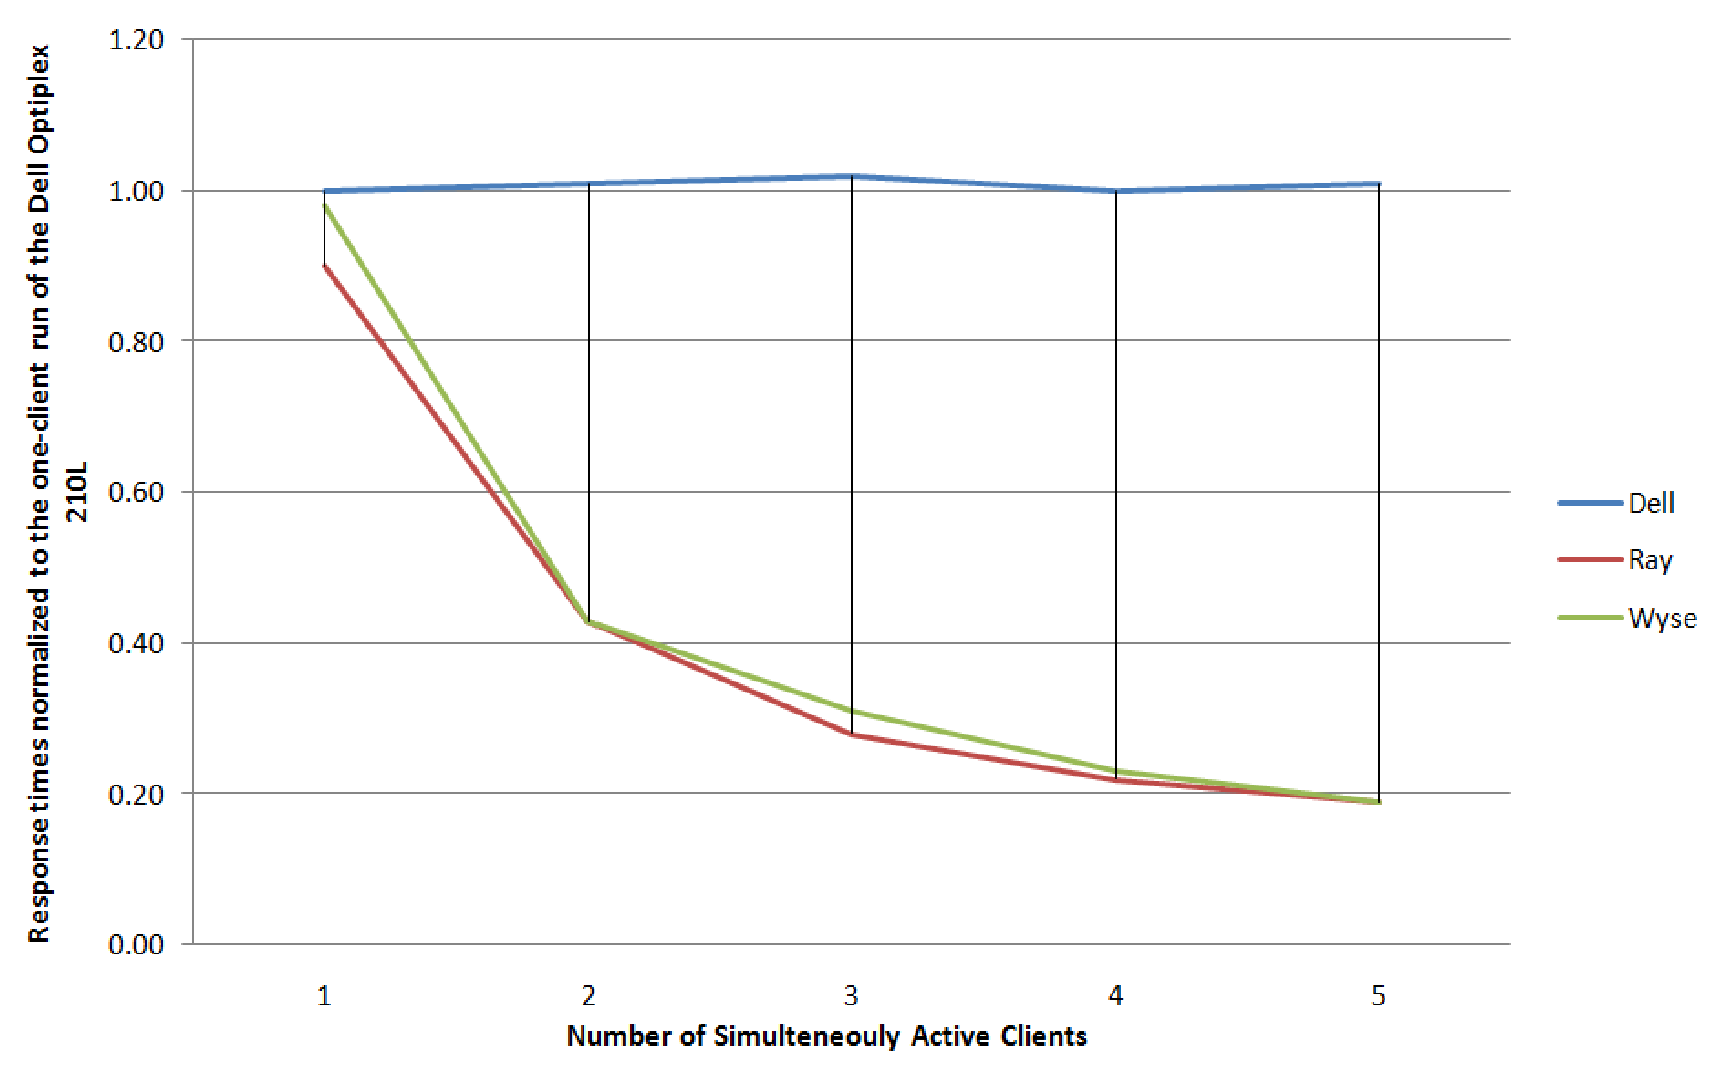
\includegraphics{graphics/graphic_excel_test}}
                    \caption{Normalized Excel Subtotals Task Response Times}
                    \label{fig:graphic_excel_test}
                \end{figure}
                \begin{table}[h!tb]
                    \centering
                    \begin{tabular}{|c|c|c|c|c|c|c|}
                    \hline
                    \multicolumn{ 3}{|c|}{Performance Results} &            & \multicolumn{ 3}{|c|}{Comparative Rating} \tn
                    \hline
                    PC solution & \multicolumn{ 2}{|c|}{Thin-client solutions} & Number of   & PC solution & \multicolumn{ 2}{|c|}{Thin-client solutions} \tn
                    \hline
                          Dell &        Sun &       Wyse & concurrent &       Dell &        Sun &       Wyse \tn

                      OptiPlex &        Ray &    Winterm &     active &   OptiPlex &        Ray &    Winterm \tn

                          210L &          2 &     5150SE &    clients &       210L &          2 &     5150SE \tn
                    \hline
                          12.9 &       13.2 &       13.1 &          1 &       1.00 &       0.90 &       0.98 \tn
                    \hline
                          12.8 &       30.2 &       29.7 &          2 &       1.01 &       0.43 &       0.43 \tn
                    \hline
                          12.7 &       45.5 &       41.9 &          3 &       1.02 &       0.28 &       0.31 \tn
                    \hline
                          12.9 &       58.3 &       57.3 &          4 &       1.00 &       0.22 &       0.23 \tn
                    \hline
                          12.8 &       68.1 &       67.9 &          5 &       1.01 &       0.19 &       0.19 \tn
                    \hline
                    \end{tabular}  
                    \captionof{table}{Performance Results for Excel Subtotals Calculation} 
                    \label{tab:table_excel_test}
                \end{table}
                \begin{figure}[h!tb]
                    \centering
                    \resizebox{\textwidth}{!}{ % Fazendo a tabela caber no espaco da pagina
                    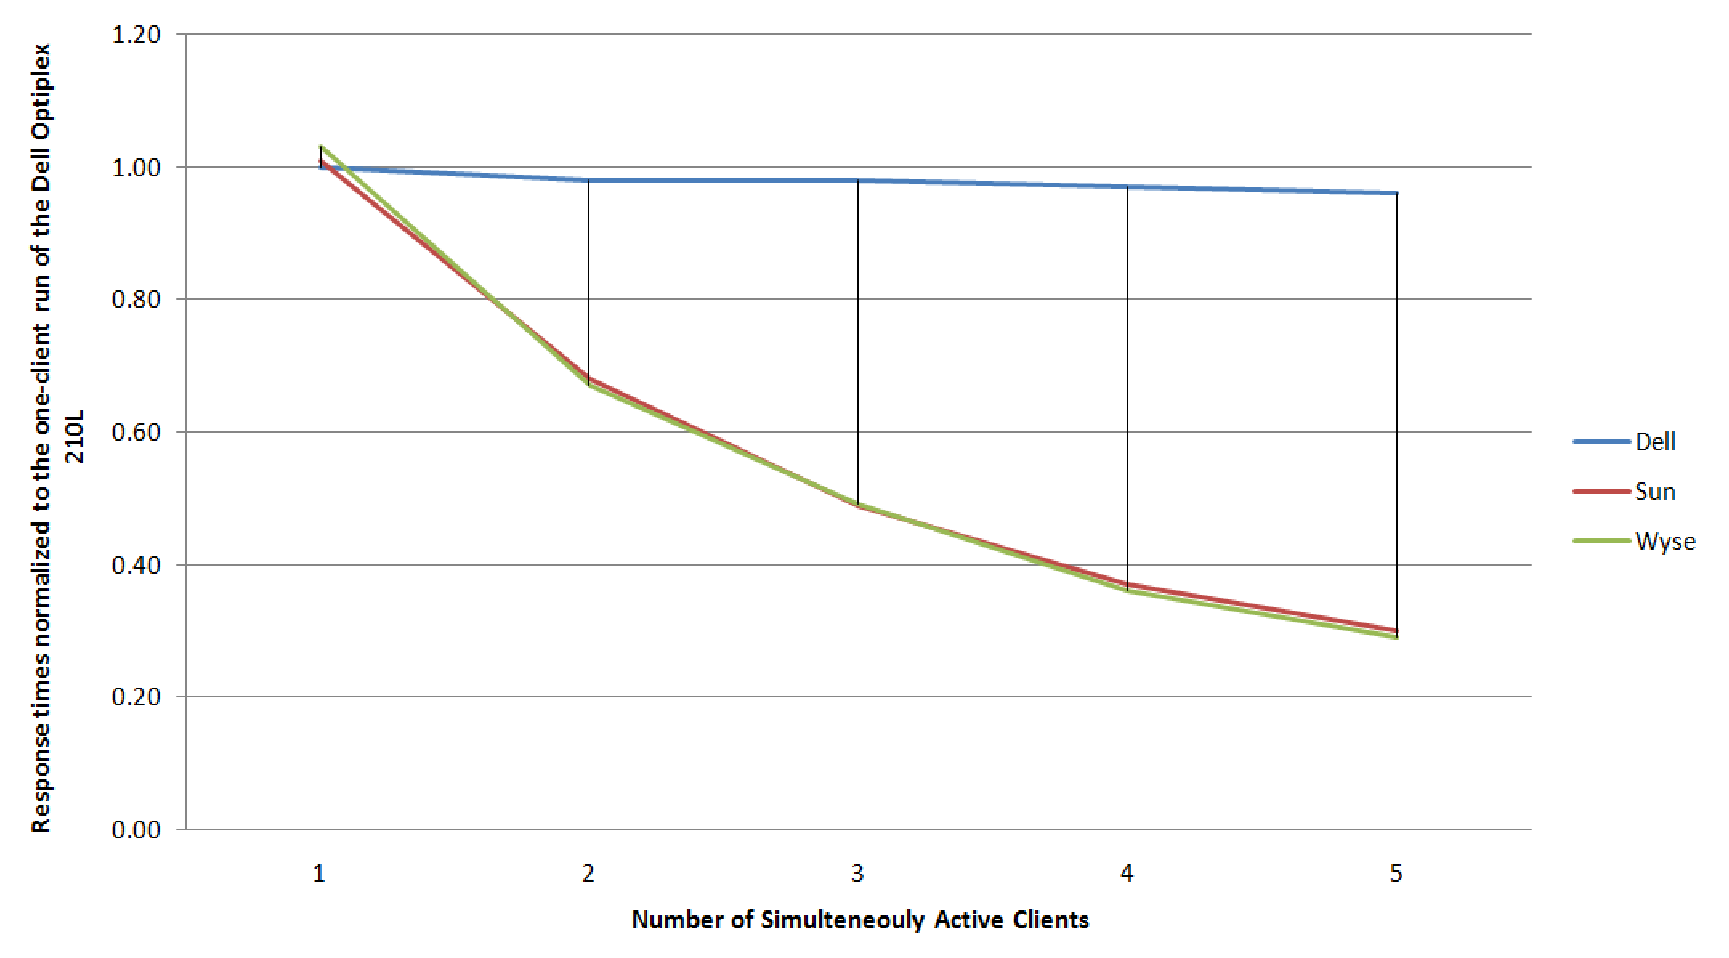
\includegraphics{graphics/graphic_pdf_test}}
                    \caption{Normalized PDF Subtotals Task Response Times}
                    \label{fig:graphic_pdf_test}
                \end{figure}
                \begin{table}[h!tb]
                    \centering
                    \begin{tabular}{|c|c|c|c|c|c|c|}
                    \hline
                    \multicolumn{ 3}{|c|}{Performance Results} &            & \multicolumn{ 3}{|c|}{Comparative Rating} \tn
                    \hline
                    PC solution & \multicolumn{ 2}{|c|}{Thin-client solutions} & Number of   & PC solution & \multicolumn{ 2}{|c|}{Thin-client solutions} \tn
                    \hline
                        Dell   &        Sun &       Wyse & concurrent &     Dell   &        Sun &       Wyse \tn

                      OptiPlex &        Ray &    Winterm &     active &   OptiPlex &        Ray &    Winterm \tn

                          210L &          2 &     5150SE &    clients &       210L &          2 &     5150SE \tn
                    \hline
                          16.1 &       16.0 &       15.6 &          1 &       1.00 &       1.01 &       1.03 \tn
                    \hline
                          16.4 &       23.8 &         24 &          2 &       0.98 &       0.68 &       0.67 \tn
                    \hline
                          16.5 &       33.0 &       33.1 &          3 &       0.98 &       0.49 &       0.49 \tn
                    \hline
                          16.6 &       43.7 &       44.3 &          4 &       0.97 &       0.37 &       0.36 \tn
                    \hline
                          16.7 &       54.0 &       55.1 &          5 &       0.96 &       0.30 &       0.29 \tn
                    \hline
                    \end{tabular}  
                    \captionof{table}{Performance Results for PDF Compression Subtotals Calculation}
                    \label{tab:table_pdf_test}
                \end{table}
                \pagebreak
            \subsubsection*{PC vs. Thin Client: Power Consumption}
                Supposing 30 thin users share a 400W server, the total power consumption will be 1300W - a yearly cost of \euro640.00. 30 PCs would consume 10000W instead - a yearly cost of \euro4900.00 (assuming the MWh cost is \euro80.00). The Table~\ref{tab:pc_thin_client_power_consumption} shows the power consumption of thin-client and PC.
                \begin{table}[h!tb]
                \centering
                    \begin{tabular}{|c|c|c|}
                    \hline
                         & {\bf Thin Client} &   {\bf PC} \tn
                    \hline
                    {\bf Weight} & 2.2 - 7.7 lbs & 22 - 33 lbs \tn
                    \hline
                    {\bf Volume} & 1.5 - 3 dm$^3$ & 30 - 35 dm$^3$ \tn
                    \hline
                    {\bf Packing material} & 2.2 - 4.4 lbs &   3 - 5 kg \tn
                    \hline
                    {\bf Power consumption\linebreak (including monitor)} & 20 - 50 watt & 300 - 400 watt \tn
                    \hline
                    {\bf Heat rejection} & 5 - 35 watt & 85 - 115 watt \tn
                    \hline
                    {\bf Noise level} & 0 dbA & 50 - 60 dbA \tn
                    \hline
                    \end{tabular}  
                    \captionof{table}{PC and thin client power consumption} 
                    \label{tab:pc_thin_client_power_consumption}
                \end{table}
                
            \subsubsection*{Hardware Savings}
                \paragraph*{Savings on client hardware} 
                    The economy brought by the substitution of PCs with thin clients was estimated around US\$ 208 per PC per year. The estimative considered the average prices of a PC, an adequate thin client and the PC upgrade costs every 3 years. If energy consumption is considered, the savings will be even greater.

                The following considerations were taken:
                \begin{itemize}
                    \item Thin client cost: US\$250.00 x PC cost: US\$750.00;
                    \item PC needs to be upgraded every 3 years and thin clients need to be replaced every 6 years.
                \end{itemize}
                Therefore, in a 6-year period US\$1500.00 will be spent on a PC against \$250.00 that will be spent on a thin client.

            \paragraph*{Extra server hardware costs}
                Considering that:
                \begin{itemize}
                    \item On average 30 users will need a dual processor server with 4 GB of RAM and SCSI hard disks;
                    \item A brand new server should cost around US\$4,500.00 and will depreciate on average in 3 years.
                \end{itemize}
                For 60 users, the thin client solution should out-price the PC one by US\$11,300.00 per year, excluding the administration costs of both solutions.

        \subsection{Servers and Virtualization} \label{sec2:servers_virtualization}
                        
            \subsubsection*{Rack vs. Blade}
                According to Goldworm\cite{barbAnne07}, Blade servers are a package of ``ultra-high density components including servers, storage, and communications interfaces in a pre-wired chassis with shared components such as power, cooling, and networking. In contrast to the conventional \emph{horizontal} positioning within a rack (rack mounted servers), blades are typically (though not always) installed \emph{vertically} in a blade chassis, like books in a bookshelf''. This disposition of the servers provide a high density of the components and thus performance, for example, 60 blade servers can fit in the same physical space as 42 rack-mounted servers. Another improvement reached with this type of server is the integration of a remote system management, differently form the ordinary (rack or standalone), where it is an add-on. An example of this type of server can be seen on Figure~\ref{fig:example_blade_server}. Moreover, Blade servers\footnote{\url{http://ieeexplore.ieee.org/xpl/freeabs_all.jsp?tp=&arnumber=1362591&isnumber=29851}} are computer servers designed to minimize the use of physical space. A blade enclosure, which can hold from 8 to 24 \cite{Rehn08} blade servers, provides common services such as power supply, cooling and networking thus eliminating redundancies in each individual blade server. More than 250 blade servers can be easily accommodated in a single rack. On the other hand approximately 42 servers can be accommodated to a standard rack when it comes to the other lower end servers available in the market. Whereas, rack-mounted servers are those arrange in industrial rack. A single rack is capable of holding 10 to 20 servers. Therefore, this type of servers come with rails or slides to ease inserting and removing of the components\cite{Bailey09}.
            \begin{figure}[h!tb]
                \centering
                \subfloat[IBM LS20]{
                    \label{fig:ibm_ls20_blade_server}
                    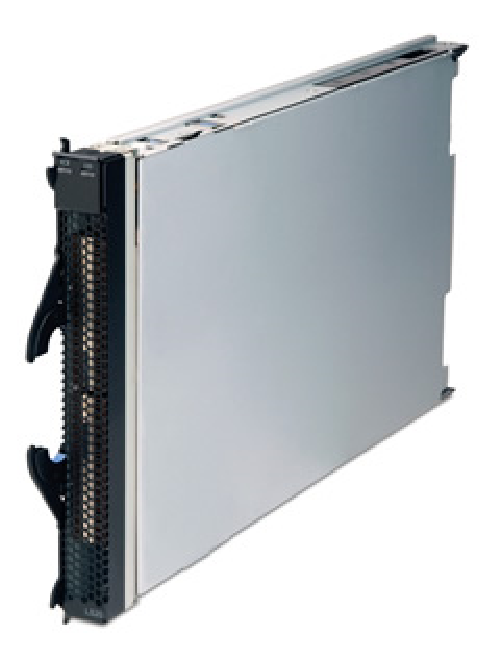
\includegraphics[width=0.3\textwidth]{graphics/ibm_ls20_blade_server}}
                \subfloat[Sun 6000 Series Blade Enclosure]{
                    \label{fig:sun_6000_blade_enclosure}
                    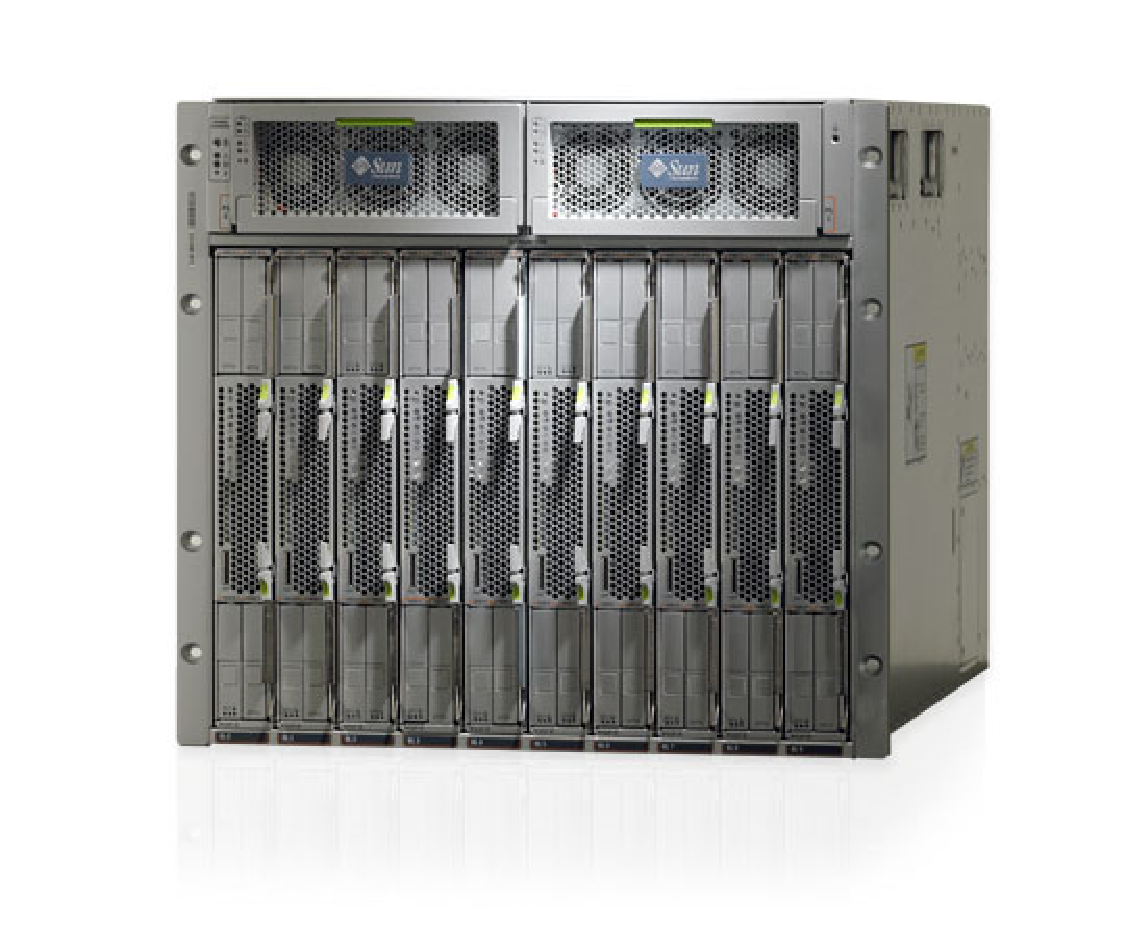
\includegraphics[width=0.3\textwidth]{graphics/sun_6000_blade_enclosure}}
                \subfloat[HP Intros Rack]{
                    \label{fig:hp_intros_blade_server_rack}
                    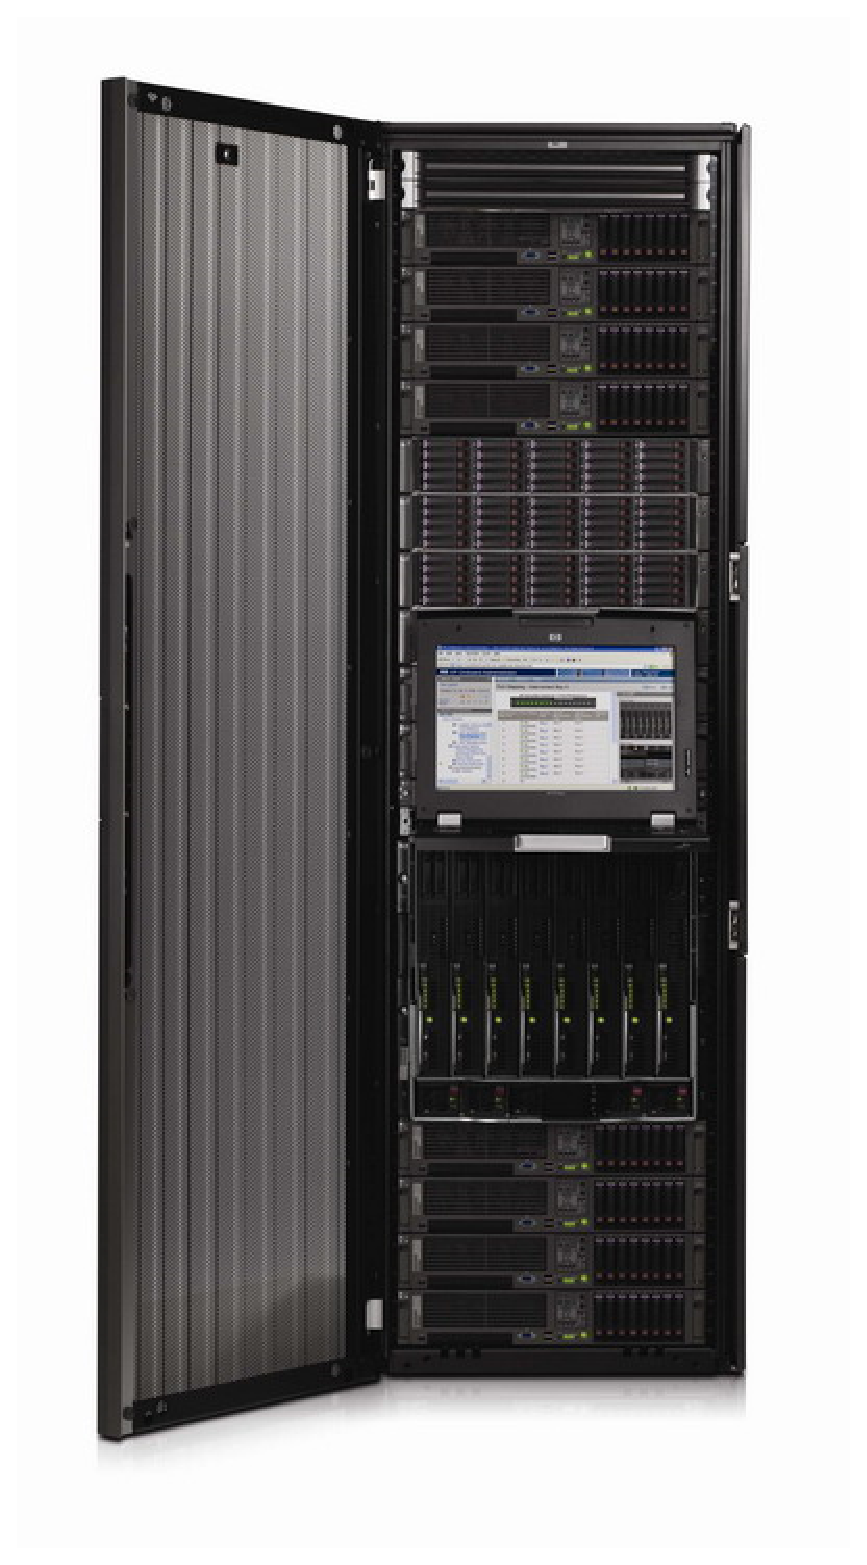
\includegraphics[width=0.3\textwidth]{graphics/hp_intros_blade_server_rack}}
                \caption{Examples of Blade Servers}
                \label{fig:example_blade_server}
            \end{figure}
            \begin{figure}[h!tb]
                \centering
                \subfloat[Chenbro 5U RM51924]{
                    \label{fig:chenbro_5urm51924}
                    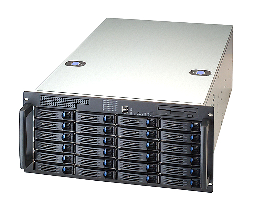
\includegraphics[width=0.3\textwidth]{graphics/chenbro_5U_RM51924}}
                \subfloat[Rack Server]{
                    \label{fig:rack_server}
                    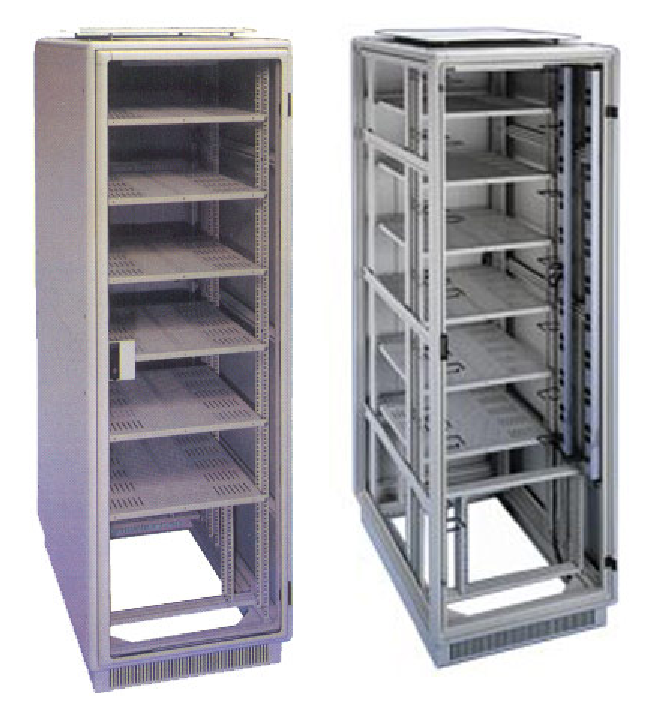
\includegraphics[width=0.3\textwidth]{graphics/rack_server}}
                \caption{Examples of Rack Servers}
                \label{fig:example_rack_server}
            \end{figure}
            In the Table~\ref{tab:power_consumption_several_servers}, a comparison is made between IBM HS21 blades and x3550 rack servers. The blades and rack servers have comparable performance.
            \begin{itemize}
                \item 2.0 GHz intel quad core;
                \item 8 GB DDR2 memory;
                \item Both in standard configuration, with no HDDs.
            \end{itemize}
            \begin{table}[h!tb]
                \centering
                \begin{tabular}{|c|c|c|c|}
                \hline
                \multicolumn{ 1}{|c|}{{\bf IBM server model}} & \multicolumn{ 1}{|c|}{{\bf Base Power}} & \multicolumn{ 1}{|c|}{{\bf kWh consumed}} & \multicolumn{ 1}{|c|}{{\bf Total cost }} \tn
                \multicolumn{ 1}{|c|}{{\bf }} & \multicolumn{ 1}{|c|}{{\bf Consumption}} & \multicolumn{ 1}{|c|}{{\bf over 5 years}} & \multicolumn{ 1}{|c|}{{\bf (\$0.03/kWh)}} \tn
                \multicolumn{ 1}{|c|}{{\bf }} & \multicolumn{ 1}{|c|}{{\bf }} & \multicolumn{ 1}{|c|}{{\bf }} & \multicolumn{ 1}{|c|}{{\bf over 5 years}} \tn
                \hline
                BC-H Chassis, no blades & 0.510 kWh &     22,350 &  \$670.50  \tn
                \hline
                BC-H HS21 blade & 0.318 kWh &     13,936 &  \$418.08  \tn
                \hline
                x3550 server & 0.373 kWh &     16,346 &  \$490.39  \tn
                \hline
                x3650 server & 0.455 kWh &     19,940 &  \$598.20  \tn
                \hline
                BC-H chassis with 14 & 4.962 kWh &    217,455 & \$6,523.65  \tn
                HS21 blades &  &  &  \tn
                \hline
                14 x3550 servers & 5.222 kWh &    228,849 & \$6,865.46 \tn
                \hline
                14 x3650 servers & 6.370 kWh &    279,259 & \$8,374.80  \tn
                \hline
                \end{tabular}  
                \captionof{table}{Power consumption for several servers, excluding cooling and redundancy}%XXX colocar referencia
                \label{tab:power_consumption_several_servers}
            \end{table}
            Thus, a possible conclusion to this comparison is that with Blade servers the gain with space, performance and, more importantly, power consumption is much smaller than with Rack-mounted devices.
            \begin{itemize}
                \item Space saving and efficiency - packaging more computer power in a significantly smaller area;
                \item Consolidation of servers to improve and centralize management as well as utilization;
                \item Return on investment (ROI) and improved total cost of ownership (TOC) through increased hardware utilization and reduced operating expenses;
                \item More energy efficient, due to existence of centralized power supply, cooling and networking.
            \end{itemize}
            According to the figures, the choice of using a blade server provides roughly 5\% power saving over a similar rack-mount configuration. The main benefit brought by the use of blade servers, however, is the processing density, as a rack filled with blade servers may carry up to 50\% more servers than one with rackable servers. Other benefits are that blade servers are easier to service and reduce the number of power cables needed from as many as 80\% \cite{Hendenson07}. 
            
            However, the high power density might prove to be a problem to server farms in terms of overheating.%XXX falar disso na parte de cooling...
            
            \subsubsection*{Virtualization}
                The overall goal of virtualization is to create a logical abstraction of physical assets. It allows to multiple ``virtual'' servers to run on one physical server, thereby consolidating many physical servers onto one. \emph{Wikipedia}, in 2009, defines virtualization as the following: ``Virtualization is the process of presenting a logical grouping or subset of computing resources so that they can be accessed in ways that give benefits over the original configuration. This new virtual \emph{view} of the resources is not restricted by the implementation, geographic location or the physical configuration of underlying resources. Commonly virtualized resources include computing power and data storage''. Moreover, virtualization improves efficiency and availability of resources and applications in the organization. According to \emph{Vmware}, it is possible to save 50-70\% overall IT costs. Overall benefits from virtualization includes: reduction of costs, free up IT resources, provide better infrastructure optimization and utilization, increase availability and improve desktop management.
                
                Regarding the energy consumption, it is a critical issue for IT organizations now a days, either the objective is the reduction of costs, environmental issues or keeping the data center running. In the United States alone, data centers consumed \$4.5 billion worth of electricity in 2006. Industry analyst Gartner \cite{GartnetKumar07} estimates that over the next 5 years, most enterprise will spend as much energy as they spend on hardware infrastructure, power and air conditioning. Besides that, virtualization has made positive improvements to the environment issue. Gartner \cite{GartnetStamford07} estimates that 1.2 million workloads run in virtual machines, which represents an aggregate power savings of about 8.5 billion kWh - more electricity than is consumed annually in all of New England for heating, ventilation and cooling. While this is a good start, there are plenty of opportunities for saving even more energy and money. Analyst firm IDC \cite{IDCDoc07} states that the un-utilized server capacity equates to approximately:
                \begin{itemize}
                    \item \$140 billion
                    \item 3 years supply of hardware
                    \item More than 20 million servers 
                \end{itemize}
                At 4 tons of carbon dioxide (CO$_{2}$) annually per server, these un-utilized servers produce a total of more than 80 million tons of CO$_{2}$ per year. This is more than is emitted from the country of Thailand and more than half of all countries in South America. In conclusion to all of these exploited data, all of these data shows that virtualization is a good improvement to the data center, saving not only space provided to the servers, but also saving energy by reducing the idle time of the server by augmenting the workload and the up-time. It is also important to state that, by providing a virtualized solution, the number and variety of applications running can be increased.

                There are two kinds of virtualization that may be used in a data center: storage and computing virtualization. Storage-area networks (SAN) may be implemented to present several different physical storage racks as a single virtual storage pool \cite{Antonopoulos05}. On the other hand, computing virtualization It can be implemented in two ways. The first case is when single physical server can offer multiple virtual servers, each with its own OS. Another option is to consolidate multiple physical servers into a cluster that acts as a single server. There are cross-platform server virtualization software available which allows data center managers to cluster and partition servers.
                \begin{figure}[h!tb]
                    \centering
                    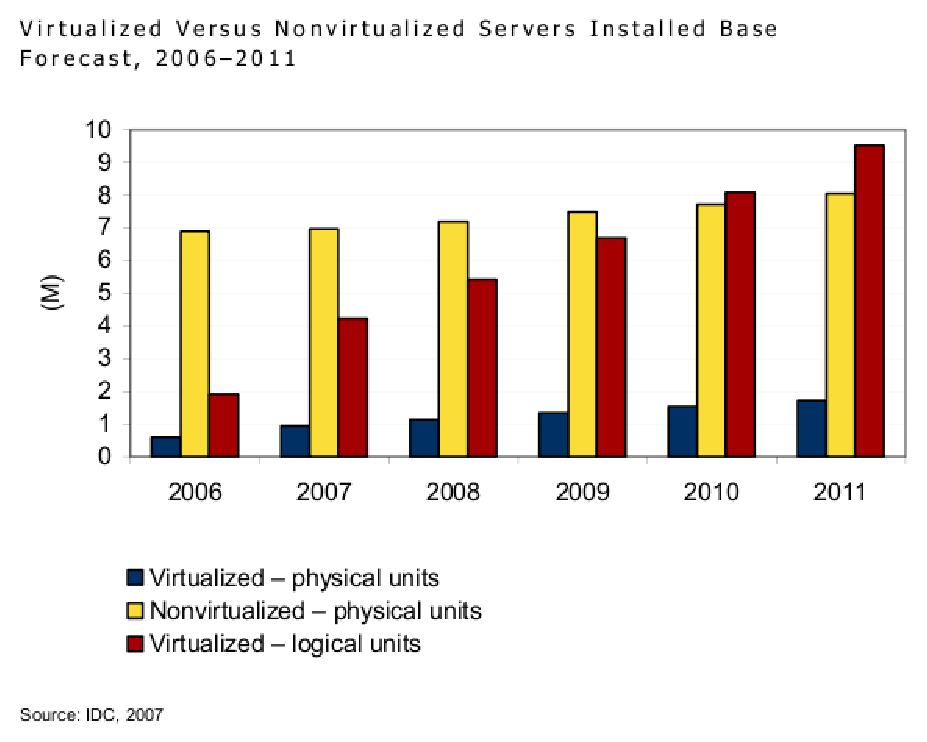
\includegraphics{graphics/installed_base_virtualized_servers}
                    \caption{Installed Base of Virtualized and Non-Virtualized Servers}
                    \label{fig:installed_base_virtualized_servers}
                \end{figure}
                
                According to the Figure~\ref{fig:installed_base_virtualized_servers} there is a trend indicating an increasing number of virtualized units over time along a forecast that by the end of 2009 the number of virtualized servers will be greater than non-virtualized ones. Logical units represent virtualized storage while physical units represent the use of non-virtualized storage. As shown in the Figure~\ref{fig:illustration_virtualization_to_physical_server}, virtualization tools such as VMware allow one physical server to act as a number of logical servers. VMware also provides a benchmark tool called VMmark\footnote{\url{http://www.vmware.com/products/vmmark/}} along with a set of test results in \cite{Makhija06} for a configuration that includes a mail server, a java server, a standby server, a web server, a database server and a file server.
                \begin{figure}[h!tb]
                    \centering
                    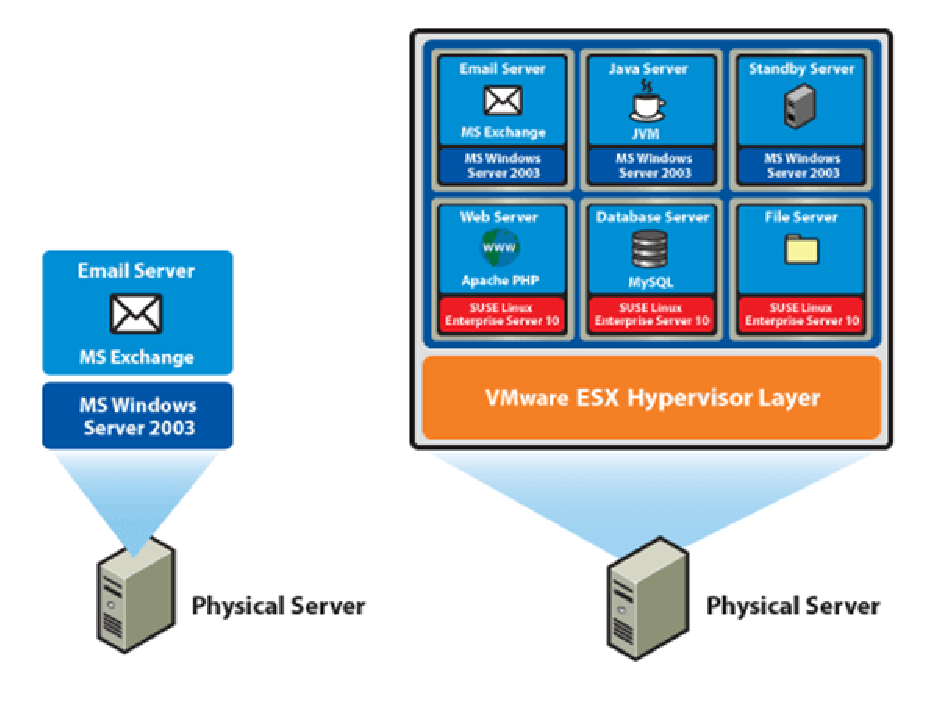
\includegraphics[scale=0.7]{graphics/illustration_virtualization_to_physical_server}
                    \caption{Illustration of Virtualization Applied to a Physical Server}
                    \label{fig:illustration_virtualization_to_physical_server}
                \end{figure}
                
                Coming along with the virtualization trend are high-throughput and eco-responsible processors such as the Sun's UltraSPARC T1 processor \cite{Hetherington05}, which support up to 128 virtualized systems in a single server and gives one of the best performance per watt of the available processors. As shown in the Table~\ref{tab:performance_power_dissipation_several_processors}\footnote{\url{http://www.anandtech.com/cpuchipsets/showdoc.aspx?i=2657&p=4}}, with relation to the UltraSPARC CPU the only comparable performance was met by the POWER5+ processor, which in average dissipates 4.5 times as much as the earlier.
                \begin{table}[h!tb]
                    \centering
                    \begin{tabular}{|c|c|c|c|c|c|c|}
                    \hline
                          &            & {\bf Power}       &                & {\bf Number}  &           &  \tn
                        &            & {\bf Dissipation} &                & {\bf of}      &           &  \tn
                        &            & {\bf CPUs}        & {\bf Number}   & {\bf Active}  & {\bf Score}   & {\bf Score} \tn
                  {\bf System} & {\bf CPU} & {\bf (Estimated)} & {\bf of cores} & {\bf Threads} & {\bf (bops)} & {\bf (\%)} \tnhl
                    Sun Fire  &  1x 1.2GHz &    72-79 W &          8 &         32 &     63.378 &      160\% \tn
                    T2000 & UltraSPARC T1 &            &            &            &            &            \tnhl
                    Sun Fire  &  2x 2.4GHz &  150-180 W &          4 &          4 &     45.124 &      114\% \tn
                    X4200 & DC Opteron &            &            &            &            &            \tnhl
                    IBM &  2x 1.9GHz &  320-360 W &          4 &          8 &     61.789 &      156\% \tn
                    p5 550 &    POWER5+ &            &            &            &            &            \tnhl
                    IBM 346 & 2x 2.8GHz  &  270-300 W &          4 &          8 &     39.585 &      100\% \tn
                    xSeries &    DC Xeon &            &            &            &            &            \tnhl
                    \end{tabular}
                    \captionof{table}{Performance and Power Dissipation for Several Processors by the Specjbb2005 Java Benchmark}
                    \label{tab:performance_power_dissipation_several_processors}
                \end{table}
                
        \subsection{Data Storage} \label{sec2:data_storage}
            Data Storage \ldots
            
            \subsubsection*{Tape Drives}
                A tape drive is a data storage device that reads and writes data stored on a magnetic tape. Its main use is as archival storage of data stored in hard drives. It is typically used for archival storage of data stored on hard drives. 
Tape media generally has a favorable unit cost; long archival stability and low energy consumption per MB of data stored to compensate for their slow seek times. Despite the slow seek time, tape drives can stream data to tape as quickly as hard drives. For example, modern LTO drives can reach continuous data transfer rates of up to 80MB/s, which is as fast as most 10,000rpm hard disks, according to \emph{Wikipedia, 2008}. Tape drives can range in capacity from a few megabytes to hundreds of gigabytes. Data can be compressed as to maximize the capacity usage. The compression rate is of usually 2:1. A set of tables related to tape drives can be found in Appendix~\ref{app:comparison_tape_drives}
            
            \subsubsection*{Disk Arrays}
                Disk array refers to a linked group of one or more physical independent hard disk constituting a larger, high-performance system. They are usually implemented using RAID technology, which can provide component redundancy and high throughputs.
        
            \subsubsection*{Comparison between Tape Drives and Disk Arrays}
                Supposing a 995 TB database consisting of:
                \begin{itemize}
                	\item Storage base (frequently used data)
                	\item Backup cache (13 weeks)
                	\item Backup archive (1 year backup)
                \end{itemize}
                A solution consisting exclusively of disk arrays would require four 32-drawer disk array systems of 245 TB each would be necessary. In order to ensure reliability and recoverability, a RAID5 format with two RAID5 arrays assigned to each drawer has been assumed. The total equipment cost is estimated on US\$10.57M \cite{Reine08} and according to the following table the disk array solution consumes 98KWh per TB per year.
                \begin{table}[h!tb]
                \centering 
                \resizebox{\textwidth}{!}{ % Fazendo a tabela caber no espaco da pagina
                \begin{tabular}{|c|c|c|c|c|c|c|c|c|}
                \hline
                & & {\bf Standby} & {\bf Per} & {\bf Number} & {\bf Total} & {\bf Power} &  & {\bf Annual} \tn
                & {\bf Processor} & {\bf Power} & {\bf SATA} & {\bf of SATA} & {\bf Array} &  {\bf Per} & {\bf Annual} & {\bf Cost} \tn
                {\bf Power} & {\bf Chassis} & {\bf Supply} & {\bf Drawer} & {\bf Drawers} & {\bf Power} &  {\bf Day} & {\bf Power} & US\$0.12/kWh \tnhl
                {\bf Typical} &  430 W/h &  34 W/h &  325 W/h &   32 &  11 kW/h & 264 kWh & 96,360 kWh & 11,563 \tnhl
                {\bf Maximum} &  800 W/h &  300 W/h &  425 W/h &   32 &  15 kW/h & 360 kWh & 131,400 kWh &  15,768 \tnhl
                \end{tabular}}
                \captionof{table}{Tape Drive Power Costs}%XXX verificar nome da tabela
                \label{tab:tape_drive_power_costs} %XXX verificar nome da tabela
                \end{table}
                With a native capacity of 800GB and throughput of 120 MB/sec, an LTO 4 drive has a compressed capability to write at 240 MB/sec, or 864 GB/hour. Supposing the same database is to be entirely stored at this drive, the equipment cost would be of US\$233,878.00 with an annual energy cost of US\$599.00.The tape solution will consume 1150 kWh in 1 year or 1,16kWh per TB per year.
                \begin{table}[h!tb]
                \centering 
                \resizebox{\textwidth}{!}{ % Fazendo a tabela caber no espaco da pagina
                \begin{tabular}{|c|c|c|c|c|c|c|c|c|}\hline
                {\bf N$^o$ of  } & {\bf N$^o$ of } & {\bf Library } & {\bf Frame} & & {\bf Drive} &  &   &  \tn
                {\bf frames} & {\bf drives } & {\bf acquisition } & {\bf acquisition } & {\bf Cartridge } & {\bf acquisition } & {\bf Space} & {\bf Energy} & {\bf Total} \tn
                {\bf acquired} & {\bf acquired} & {\bf cost} & {\bf cost} & {\bf cost} & {\bf cost} & {\bf cost} & {\bf cost} & {\bf cost} \tnhl
                1 &    2 &    76,000 &    30,000 &   82,278 &   45,600 &   68,850 &   599 &    303,327 \tnhl
                \end{tabular}}
                \captionof{table}{Disk Array Power Costs}%XXX verificar nome da tabela
                \label{tab:disk_array_power_costs} %XXX verificar nome da tabela
                \end{table}
                In overall, for the 995 TB database the following conclusions can be drawn:
                \begin{itemize}
	                \item Disk arrays consume 84 times as much as tape drives, per TB stored
	                \item The disk array solution costs 35 times as much as the tape drive solution
                \end{itemize}
                Although the cost difference between of both solutions may be high, performance should be also considered in the comparison. In that case, an adequate proportion between disk array and tape storage must be drawn according to the frequency of backup access.

        \subsection{Power Architectures} \label{sec2:power_architectures}
            \subsubsection*{Conventional AC Architecture}
                \begin{figure}[h!tb]
                    \centering
                    \resizebox{\textwidth}{!}{ % Fazendo a tabela caber no espaco da pagina
                    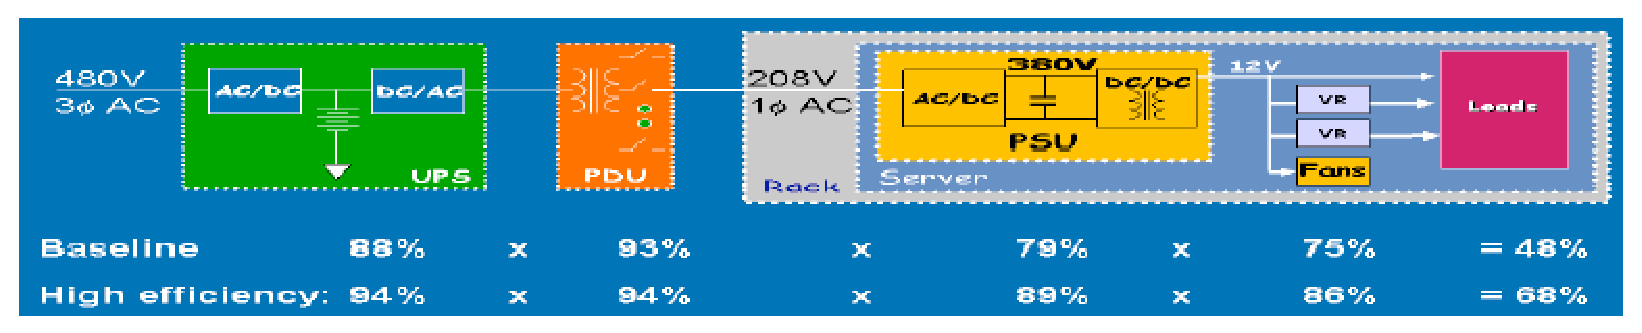
\includegraphics{graphics/conventional_ac_efficiency}}
                    \caption{Conventional AC architecture efficiency}
                    \label{fig:conventional_ac_efficiency}
                \end{figure}
                In this configuration (Figure~\ref{fig:conventional_ac_efficiency})the following transformations take place:
                \begin{itemize}
	                \item PDU steps down the voltage from 480VAC to 208VAC;
                    \item Power Supply Unit (PSU) converts 208VAC to 380VDC;
                    \item Final component distribution at 12VDC.
                \end{itemize}
                The efficiency is measured for both conventional (baseline) and high efficiency (best-in-class) equipments. The difference in efficiency between the two equipment choices is of 20\%.

            \subsubsection*{Rack-Level DC Architecture}
                \begin{figure}[h!tb]
                    \centering
                    \resizebox{\textwidth}{!}{ % Fazendo a tabela caber no espaco da pagina
                    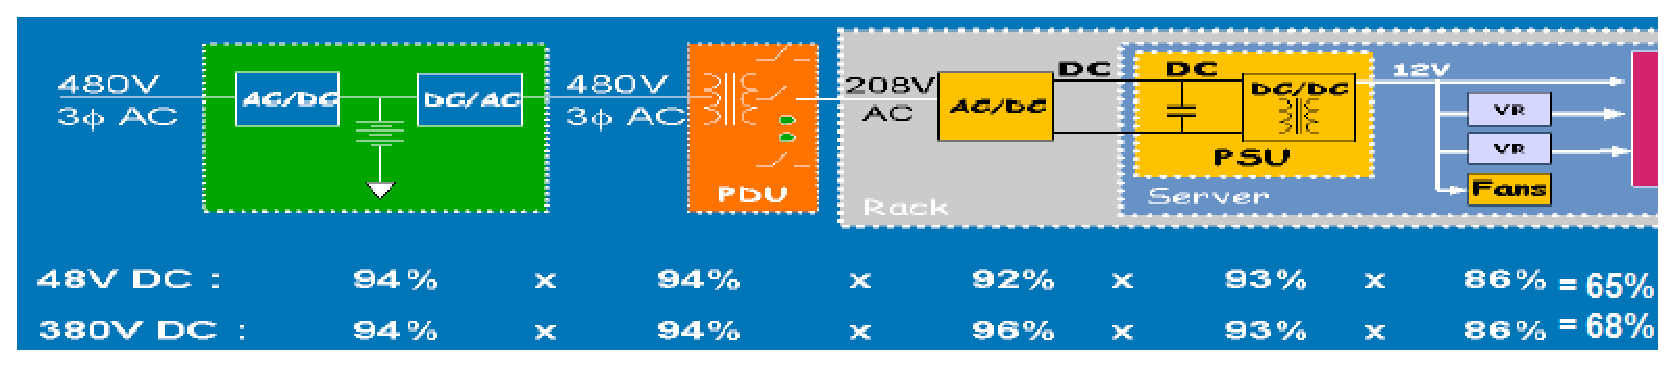
\includegraphics{graphics/rack_level_dc_efficiency}}
                    \caption{Rack-level DC architecture efficiency}
                    \label{fig:rack_level_dc_efficiency}
                \end{figure}
                On Figure~\ref{fig:rack_level_dc_efficiency}, it is possible to see that, after the PDU, an 208VAC to 48VDC/380VDC conversion is made in the rack. PSU and PDU are considered to be best-in-class, with high efficiency.

            \subsubsection*{Facility-level DC Architecture}
                \begin{figure}[h!tb]
                    \centering
                    \resizebox{\textwidth}{!}{ % Fazendo a tabela caber no espaco da pagina
                    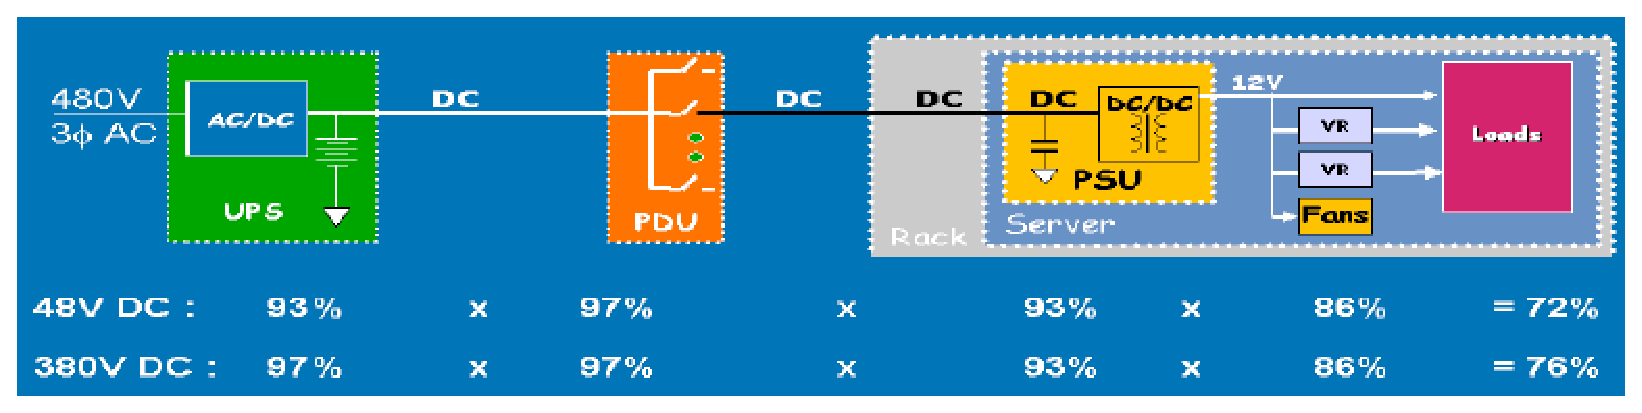
\includegraphics{graphics/facility_level_dc_efficiency}}
                    \caption{Facility-level DC architecture efficiency}
                    \label{fig:facility_level_dc_efficiency}
                \end{figure}
                In this configuration (Figure~\ref{fig:facility_level_dc_efficiency}), the DC-AC conversion in the UPS and the AC-DC conversion in the power supply are removed. It can be noted that the 480VAC-380VDC conversion in the UPS is more efficient than the 480VAC-48VDC conversion.
            
        \subsection{Data Center Infrastructure} \label{sec2:data_center_infrastructure}
            \subsubsection*{Water Cooling}%TODO
                The reasonable limit of rack power and cooling capacity for a conventional forced-air (HVAC) cooled data center is 8 kW per rack. For power densities approaching 15 kW per rack, the layout of the computing rooms and cooling facilities must be determined using specialized software (such as HP Static Smart Cooling). For racks requiring more than 15 kW, the latest cooling techniques use water (Figure~\ref{fig:power_consumption_number_servers_rack}) \cite{HPCooling07}.
                \begin{figure}[h!tb]
                    \centering
                    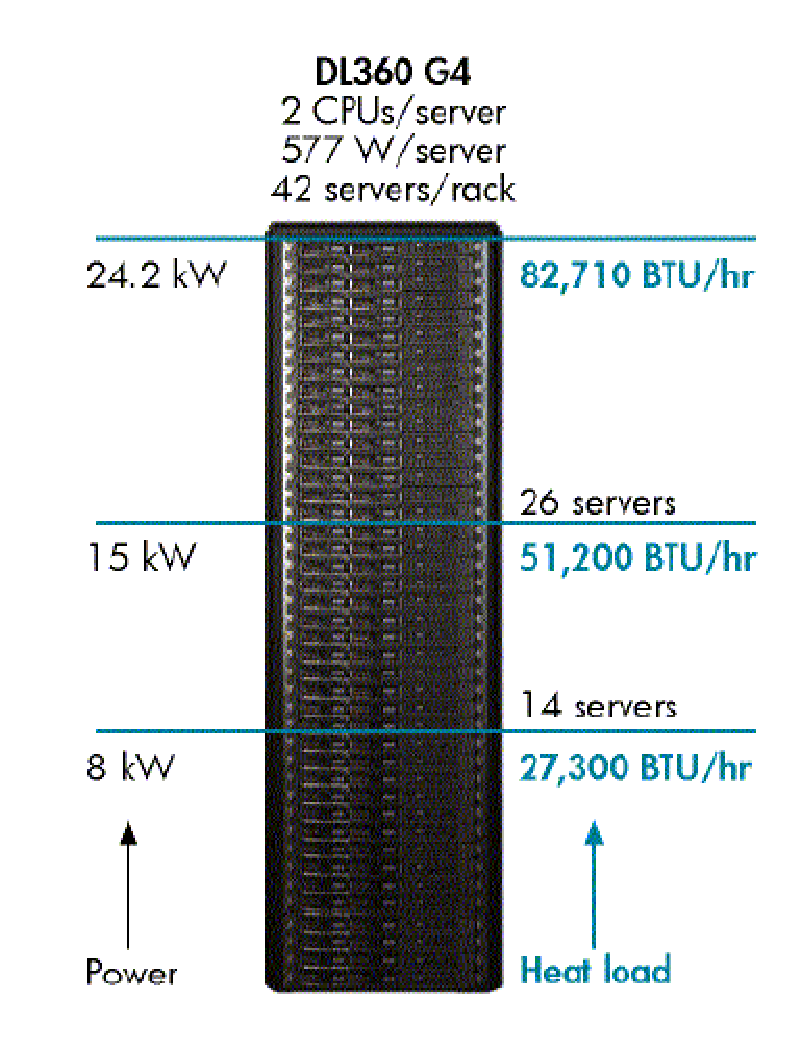
\includegraphics[scale=0.5]{graphics/power_consumption_number_servers_rack}
                    \caption{Power Consumption per Number of Servers in the Rack}
                    \label{fig:power_consumption_number_servers_rack}
                \end{figure}
                As shown in the following figure, the use of water cooling reduces in 50\% the equipment footprint, allowing greater server density. A 35 kW heat load dispersed among 4 racks could be concentrated in one single rack.
                \begin{figure}[h!tb]
                    \centering
                    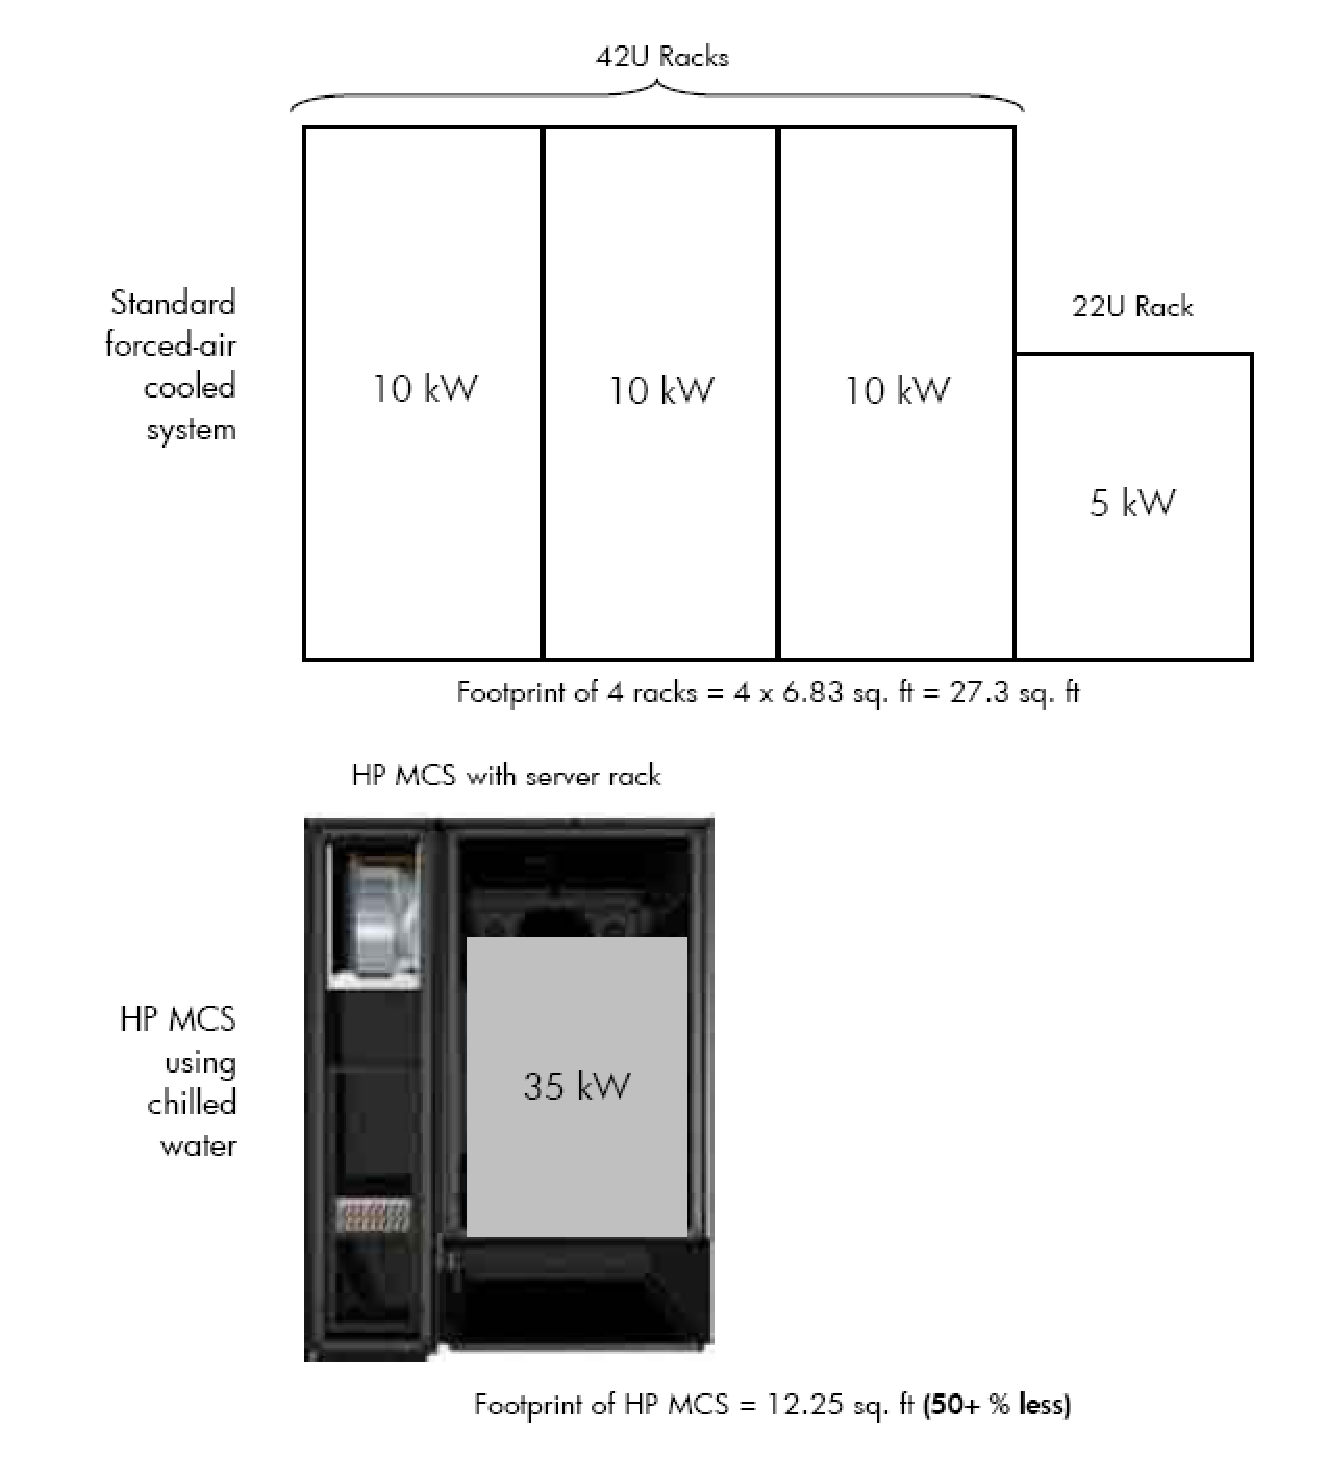
\includegraphics[scale=0.5]{graphics/footprint_reduction_for_35_heat_load}
                    \caption{Footprint Reduction for a 35 kW Heat Load}
                    \label{fig:footprint_reduction_for_35_heat_load}
                \end{figure}
                With relation to maintenance costs, Figure~\ref{fig:economic_crossover_annualized} \cite{}
                \begin{figure}[h!tb]
                    \centering
                    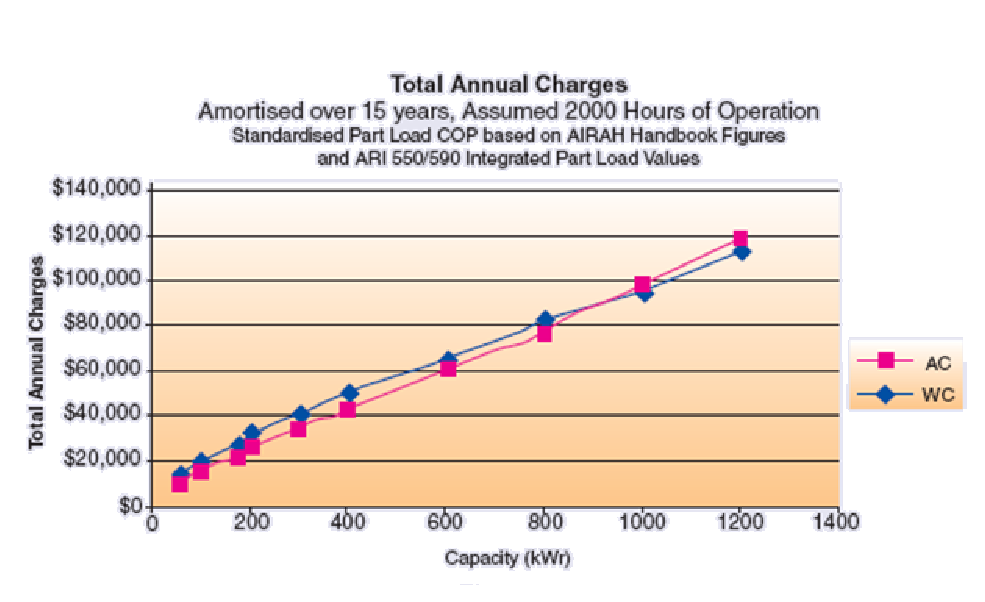
\includegraphics[scale=0.8]{graphics/economic_crossover_annualized}
                    \caption{Economic Cross-over of Annualized Charges Air-cooled to Water-cooled for 2000 Hours of Operations (in US \$)}
                    \label{fig:economic_crossover_annualized}
                \end{figure}
                \begin{figure}[h!tb]
                    \centering
                    \resizebox{\textwidth}{!}{ % Fazendo a tabela caber no espaco da pagina
                    \includegraphics[scale=0.5]{graphics/life_cycle_costs_water_cooled_air_cooled}}
                    \captionof{table}{Life Cycle Costs of Water-cooled and Air-cooled Solutions}
                    \label{tab:life_cycle_costs_water_cooled_air_cooled}
                \end{figure}
                The annual costs for water cooling and air cooling (including charges, maintenance, equipment) do not differ by a large amount. The main benefit from water cooling is the footprint reduction which can increase the server density in a datacenter%TODO

\pagebreak%XXX coloquei um pagebreak aqui, tirar depois.
\section{Green ICT or Green Computing} \label{sec2:green_ict}
% TODO
    Green ICT is a new term originated from ``Green Computing'', it is the research and development environmental impact related projects, making use of Information and Communication Technology and related applications or softwares in order to monitor the climate changes by a sustainable evolution. With that, it is possible to know how to make a responsible use of computers and related resources. It is a new paradigm that has the objective in the environment. In order to achieve this objective, it is necessary to understand and have the ability to analyze the information about the ICT components among workstations, servers, network, cooling and many others. 
    
    Furthermore, It is also important to consider that there are some indirect objectives concerning green computing. Such objectives includes reduction of costs, reduction of carbon footprint and disposal of hazard elements to the environment. The reduction of costs is provided by the fact that if the energy consumed by the components is reduced, the payment in the electricity bill is directly reduced, also, when by applying the well management of the resources, the costs related to cooling, the space required for the data center and the efficiency of the computer components are all indirectly reduced.
    
    In the section~\ref{sec2:energy_categories} is explained all the approaches and categories for applying a green solution.
    

    
\section{Devices Consumption} \label{sec2:devices_consumption} 
% TODO
    
\section{Measurement Tools} \label{sec2:tools}
% TODO


